\documentclass{sigchi}



% Load basic packages
\usepackage{balance}       % to better equalize the last page
\usepackage{graphics}      % for EPS, load graphicx instead 
\usepackage[T1]{fontenc}   % for umlauts and other diaeresis
\usepackage{txfonts}
\usepackage{mathptmx}
\usepackage[pdflang={en-US},pdftex]{hyperref}
\usepackage{color}
\usepackage{booktabs}
\usepackage{textcomp}

% Some optional stuff you might like/need.
\usepackage{microtype}        % Improved Tracking and Kerning
% \usepackage[all]{hypcap}    % Fixes bug in hyperref caption linking
\usepackage{ccicons}          % Cite your images correctly!
% \usepackage[utf8]{inputenc} % for a UTF8 editor only

% If you want to use todo notes, marginpars etc. during creation of
% your draft document, you have to enable the "chi_draft" option for
% the document class. To do this, change the very first line to:
% "\documentclass[chi_draft]{sigchi}". You can then place todo notes
% by using the "\todo{...}"  command. Make sure to disable the draft
% option again before submitting your final document.
\usepackage{todonotes}

% Paper metadata (use plain text, for PDF inclusion and later
% re-using, if desired).  Use \emtpyauthor when submitting for review
% so you remain anonymous.
\def\plaintitle{Adaptive Project Planning for Epics, Features, and User Stories in Modern Software Develop Management}
\def\plainauthor{First Author, Second Author, Third Author,
  Fourth Author, Fifth Author, Sixth Author}
\def\emptyauthor{}
\def\plainkeywords{Adaptive Project Planning; Agile Software Development.}
\def\plaingeneralterms{Documentation, Standardization}

% llt: Define a global style for URLs, rather that the default one
\makeatletter
\def\url@leostyle{%
  \@ifundefined{selectfont}{
    \def\UrlFont{\sf}
  }{
    \def\UrlFont{\small\bf\ttfamily}
  }}
\makeatother
\urlstyle{leo}

% To make various LaTeX processors do the right thing with page size.
\def\pprw{8.5in}
\def\pprh{11in}
\special{papersize=\pprw,\pprh}
\setlength{\paperwidth}{\pprw}
\setlength{\paperheight}{\pprh}
\setlength{\pdfpagewidth}{\pprw}
\setlength{\pdfpageheight}{\pprh}

% Make sure hyperref comes last of your loaded packages, to give it a
% fighting chance of not being over-written, since its job is to
% redefine many LaTeX commands.
\definecolor{linkColor}{RGB}{6,125,233}
\hypersetup{%
  pdftitle={\plaintitle},
% Use \plainauthor for final version.
%  pdfauthor={\plainauthor},
  pdfauthor={\emptyauthor},
  pdfkeywords={\plainkeywords},
  pdfdisplaydoctitle=true, % For Accessibility
  bookmarksnumbered,
  pdfstartview={FitH},
  colorlinks,
  citecolor=black,
  filecolor=black,
  linkcolor=black,
  urlcolor=linkColor,
  breaklinks=true,
  hypertexnames=false
}

% create a shortcut to typeset table headings
% \newcommand\tabhead[1]{\small\textbf{#1}}

% End of preamble. Here it comes the document.
\begin{document}

\title{\plaintitle}

\numberofauthors{3}
\author{%
  \alignauthor{Baoshu Feng\\
    \affaddr{Chicago, Illinois}\\
    \affaddr{A20343813}\\
    \email{bfeng7@hawk.iit.edu}}\\
}

\maketitle

\begin{abstract}
  Modern software engineering development projects are usually embedded in a dynamic environment. The dynamic environment involves a high degree of uncertainty and includes many unpredictable components, such as stakeholders, changes in demand, and budget control. Managing projects under complex and uncertain conditions challenge the team's creativity and adaptability. Because traditional engineering project management methods cannot fully adapt to dynamic environments, software engineering management requires highly adaptable project planning and management models, also known as "Agile" Project Management. User stories are often misunderstood as small bits of requirements that help postpone analysis, but that’s not what adaptive planning should be about. Adaptive plans help organizations turn a changing landscape into a competitive advantage, react faster than the market and accelerate product discovery. This paper investigates the use of adaptive project planning techniques for software development management, including XP and Scrum.
\end{abstract}



\begin{CCSXML}
<ccs2012>
   <concept>
       <concept_id>10011007.10011074.10011092.10011096.10011097</concept_id>
       <concept_desc>Software and its engineering~Software product lines</concept_desc>
       <concept_significance>500</concept_significance>
       </concept>
 </ccs2012>
\end{CCSXML}

\ccsdesc[500]{Software and its engineering~Software product lines}

% Author Keywords
\keywords{\plainkeywords}

% Print the classficiation codes
\printccsdesc



\section{Introduction}
Lack of consistency is a typical feature in the software development process. Since software engineering is made up of many short-term decisions, this strategy works well for small systems. As the system grows, adding features becomes complicated, and errors become common and difficult to fix. This primitive decision-making mode requires a long system test phase, but testing and debugging is challenging to arrange. Therefore, a strict plan-driven introduction of software development engineering. Plan-driven software development is more predictable and more efficient. The plan-driven approach is widely used in traditional engineering fields, but the plan-driven paradigm is not fully applicable in software development engineering. The speed of software development is reduced due to rigid processes and cannot adapt to the dynamic development environment. 

Adaptive project management, as known "agile method", is created in response to the shortcomings of plan-driven project management mentioned above. Adaptive project management is a compromise between no process and too many processes. Plan-driven project management is document-oriented. Adaptive project management is code-oriented.
\begin{enumerate}
\item On the one hand, plan-driven project management is predictive. Therefore, the plan-driven approach tends to make detailed plans for a long period of time in the future. The plan-driven approach expects that the effectiveness of the plan can be sustained. On the contrary, adaptive project management is more friendly to future changes.
\item On the other hand, adaptive project management emphasizes the skills of the development team rather than the importance of detailed processes.
\end{enumerate}

Adaptive project management completes the trade-off between development efficiency and the ease of control, and provides reasonable returns for the project.

User stories are short, simple descriptions of a feature told from the perspective of the person who desires the new feature. User stories can be written at varying levels of detail. Thus, user stories can be written to cover large amounts of features. These are generally known as epics. Epics are generally too large to complete in one agile iteration. It is split into smaller user stories. With adaptive project planning, developer is highly efficient to design and implement features, user stories and epics [5].


\section{Discussion}


\subsection{5 Typical Adaptive Project Management Approaches }

Project managers will produce a delivery plan when the project tasks are agreed upon. Project managers can plan the project on the premise that changes under the pressure of technical infeasibility are ignored. This process is summarized into seven steps to build people, processes, and products to achieve the mission. Figure 1 shows this process. This process includes C-Constraints, P-Products (outputs), P-Processes (tasks), R-Resources, R-Risks, S-Schedule, S-Stakeholders. A process is a list of tasks that can provide you with products. Products are about the outputs you need to achieve the outcomes. Resources are the capabilities required to complete the task. Risk is a factor that threatens the realization of goals. A schedule is an orderly time series of activities of a resource. Stakeholders are the views on whether the plan is acceptable (see in Figure 1)[2].

This plan is not seen as a top-down process, a one-time process. In the adaptive planning paradigm, every step may lead to a return. Every time I return to re-examine the choices and decisions made at the upper chain. In this process, the two unchangeable things are constraints and goals. Project managers must obtain permission from the sponsor and other key stakeholders to change any of them, otherwise, they will face the real danger of destroying the critical bridge between the project’s mission model and the executable plan [2].

In the early stages of project planning, the engineer must consider the relationship between project constraints and product delivery methods. In time-constrained projects, the primary constraint on project planning is the completion speed. Although increasing the rate is more expensive and riskier than the normal process, the process will satisfy the project.

In time-constrained projects, operational processes, resource solutions, and related risks are all standard ways of doing things and may be modified to deliver project results. Innovation and creativity must be encouraged, and team members must develop new ways to achieve the expected output and results[2].

In resource-constrained projects, the project manager should determine the end date and try to ensure that there are no signal events. Because it does not follow the standard CPPRRSS planning sequence, as shown in Figure 1. Resources are tightly tied to the processes they can deploy effectively, and there is rapid iteration between them. Productivity is the key information. In this case, the clearance rate is important (see in Figure 1). The deciding factor in determining the completion date is the signal clearance rate, which is performed by first-principles signal engineers and can only be performed by first-principles signal engineers, and their availability limits throughput. This kind of insight stops the planning process because it can lead the project on the wrong path. The project needs to be planned as a resource-constrained project. When the processes are chosen are highly skilled resources carrying out intellectually demanding tasks, project managers need to build additional temporary and management products to monitor progress.

Premature application of budget constraints in the project life cycle can lead to ineffective planning actions and unnecessary governance interventions as costs increase. Because this situation is very common, many project managers usually mention the customer's price or date, which immediately translates into a budget and end date. This strategy is used to deal with the pressure of failed budget forecasts. In project management, the governance team converts a single number estimate into a constraint. The appropriate result of the conversation about cost estimation between the sponsor and the project manager is a compromise and understanding of the different understandings of the budget between the sponsor and the project manager (see in Figure 1). A reasonable budget estimate must appropriately reflect the level of uncertainty, determine the driving factors of uncertainty, and reflect current experience based on history and trends. The correct setting of budget constraints is only a condition for the project's success.

In mission-constrained projects, risk avoidance drives planning. At the top of the hierarchy, the constraint is "quality"-it fully complies with the pre-specified capabilities. This is the usual planning process for mandatory revisions. The focus is on avoiding the possibility of unmanageable events; it is about the process of using known performance to indicate a very high level of reliability, and inevitably, it is being tested (see in Figure 1). The gold standard for testing is verification. Verification is a technique that proves that the process used is the correct process used in the correct way. Successful verification is quality assurance, which ensures that any errors that occur are known and predictable. Another method is to test through verification. 

Testing is a quality control technique that compares the performance of a product with its predicted performance, but only in those situations where the tester can think of and can find a simulation method. The project manager uses very professional knowledge to win the respect of all team members. The project manager can evaluate and prioritize the team's input. In these cases, use professional knowledge to select recommendations to listen to and make a critical judgment. By assuming responsibility for decision-making, the project manager convinces other stakeholders that they will have to do something they think has been done. In the field of software development and testing, expert status is essential for determining methods and persuading others. In a mission-constrained project, the adaptive plan for learning in the process is not applicable. It is also a risk aversion scenario for project managers to use only tried-and-tested processes to oppose innovation resolutely. If there is no process available, then the deployment of any new method will be very careful work. Prudence is a characteristic of Small and mid-size enterprises (SMEs). The expertise of SMEs is based on a disciplined approach and value system that respects previous experience and proven procedures used by other professionals [2].

The focus of more and more projects has shifted to the factors that make the project successful, such as whether it produces the right impact, creates value, and realizes sustainable value. Project managers not only need to focus on the factors of proper resource allocation for clearly defined tasks. Focusing on the delivery of results rather than outputs is achieved by focusing on a combination of Critical success factors (CSFs) and limiting factors (see in Figure 1). The project management manager needs to be aware of the importance of satisfying stakeholders and ensuring that the project's output is adopted and used. Stakeholder participation is the importance of successful project management. Project managers can no longer have confidence in the success of following a technically well-executed schedule. Project managers need to work with stakeholders and sponsors to ensure that the content delivered by the project has value in the business environment. Given this realignment of management attention, the planning process needs to respond to a redefinition of success. CSFs need to become complex to adapt to new satisfaction standards. The success factors of the project list the things we must pay attention to in planning and delivery. If CSFs cannot be implemented, the project will fail. The project customer defines the CSF. The project manager must plan and deliver the project to ensure its realization. However, the correct CSFs may be difficult to sort out from stakeholders. Because customers often make you believe that everything is related to money or that everything is associated with an end date. The review of every decision made by stakeholders clearly shows that when making a choice, they are more interested not in staying within budget or completing the schedule but in emotional value and aesthetic value. These abstract CSFs are real CSFs. Therefore, project managers need to communicate with customers carefully and in detail. This process is continuous and involves the entire life cycle of the project.


\begin{figure}
\centering
  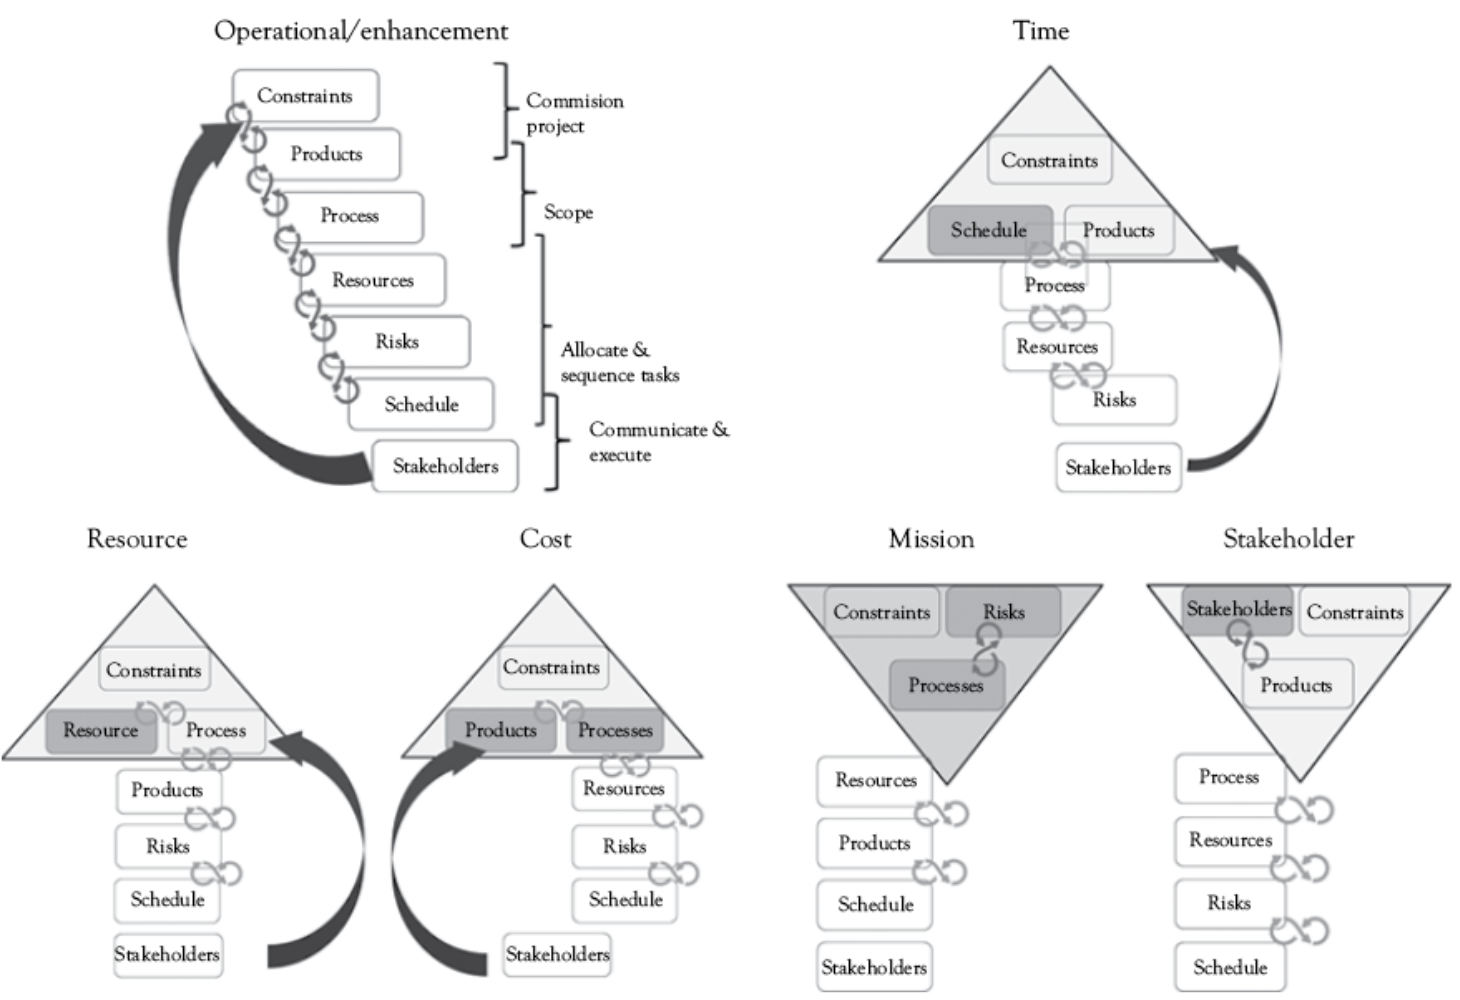
\includegraphics[width=0.9\columnwidth]{figures/approach}
  \caption{Five approach of adaptive project planning }~\label{fig:figure1}
\end{figure}


\subsection{XP and Scrum Application on Features, User Stories and Epics}

\begin{figure}
\centering
  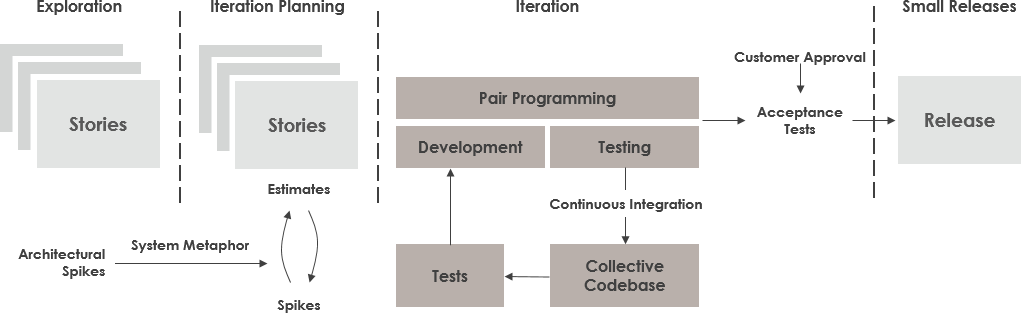
\includegraphics[width=0.9\columnwidth]{figures/xp}
  \caption{XP Application }~\label{fig:figure1}
\end{figure}

Extreme Programming (XP) starts with five values (communication, feedback, simplicity, courage, and respect). Then it is subdivided into fourteen principles and then subdivided into twenty-four practices. The idea is that practice is a specific thing that the team can do every day, and values are the basic knowledge and understanding of supporting methods (see in Figure 2). Values without practice are difficult to apply and can be applied in so many ways that it is difficult to know where to start. Valueless practice is a rote activity without a purpose. Values and practices are needed, but a big gap between them principles can help bridge this gap. Many of XP's practices are old and time-tested techniques but are often forgotten by many people, including most planning processes. In addition to resurrecting these technologies, XP also weaves them into a synergistic whole, each of which is enhanced by other technologies and given goals through values [3].

The most eye-catching thing, and one of the things that attracted me at first, is its high emphasis on testing. Although all processes mention testing, most processes don't pay much attention to it. However, XP puts testing at the foundation of development, and every programmer is writing tests when writing production code. These tests are integrated into the continuous integration and build process, thus providing a highly stable platform for future development. The XP approach is often described here under the heading of Test Driven Development (TDD), and it is influential even in other places where XP is not adopted.

\begin{figure}
\centering
  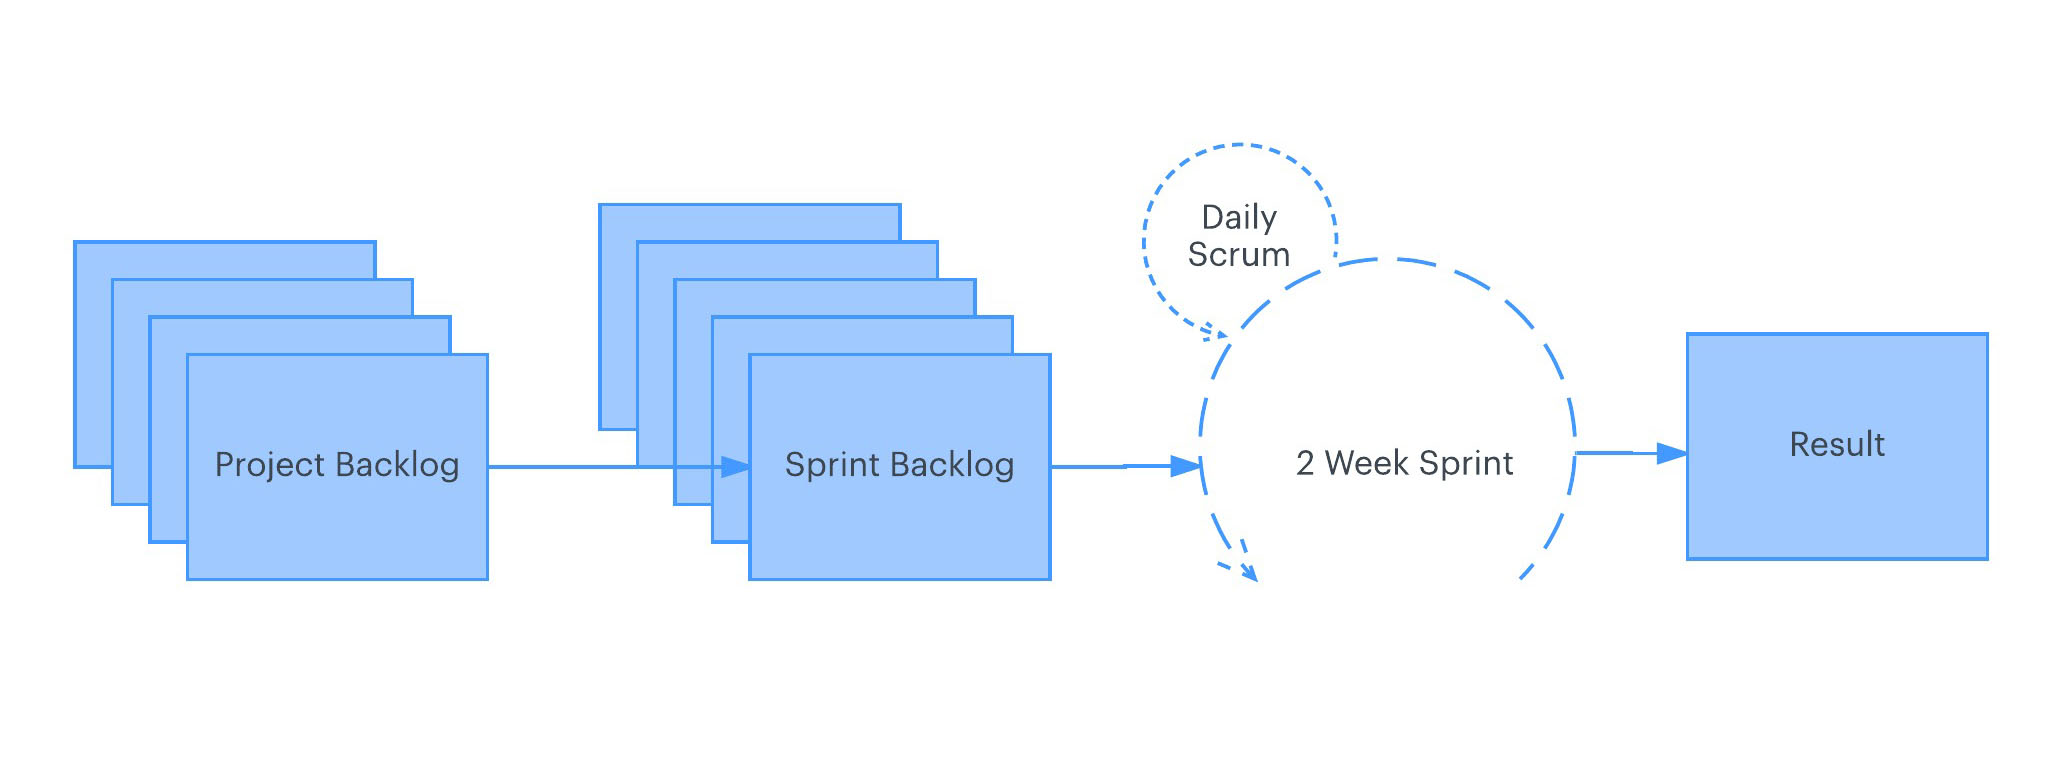
\includegraphics[width=0.9\columnwidth]{figures/scrum}
  \caption{Scrum Application }~\label{fig:figure1}
\end{figure}

Scrum focuses on the management aspect of software development, dividing development into 30-day iterations (called "sprints"), and applying closer monitoring and control through daily Scrum meetings (see in Figure 3). It pays little attention to engineering practice, and many people combine its project management methods with engineering practice of Extreme Programming. (The management practices of XP are actually not much different.)

\subsubsection{Case Study: Applying Agile Software Development on a Web Application}


XP follows KIS (Keep It Simple) principle. CRC
(Class-Responsibility- Collaborator) cards identify and
organize the object oriented classes that are relevant to
the current software increment. Design occurs both
before and after coding commences. Refactoring
means that design occurs continuously as the system is
constructed [4].

SCRUM incorporates the following framework activities.
\begin{itemize}
\begin{enumerate}
\item Requirements
\item Analysis
\item Design
\item Evolution and Delivery
\end{enumerate}

\end{itemize}
Each framework activity will have work task
occur within a process pattern called a sprint, is defined and often modify in real time by the scrum team. Scrum emphasizes the use of set of software process pattern that were proven effective for project with tight timeliness changing requirements and business criticality [4].

In agile development process by using XP methodology, the stories can be divided in two number of small depending on the time factor (if a story exceeds 3 week s for the development that can be divided in to small stories). So in XP the changes can be allowed in the middle of the development. 

For example, in this case study if we consider the legal issues, adding of another new requirement related to complaint like cybercrime will cause some change in the development which is going to have effect on the size of the story which already have been specified. These types of changes can be acceptable in XP. 

In Scrum once the sprints are identified and allotted to the team members they must be stable because they are frozen. No modifications are allowed until the completion of the development of that sprint. Adding of new sprints in the middle of the development is not possible. In XP team size should not exceed 10 members, and it is limited to 7 in scrum. XP will not support the distributed development, scrum will support [4].


\section{Conclusion}

Adaptive Project management, despite its checkered history of success, is the most influential management approach of the twentieth century, and many great things have been done using it. Gaining mastery over uncertainty by using plans to shape the world; structuring the work people do and ordering the environment to make things possible and gives a great sense of accomplishment.

Using agile methods is not for everyone. In today's environment, the most common method is coding and repairing. Applying more discipline instead of chaos will almost certainly help, and the advantage of an agile method is that it is much less than using heavyweight methods. Here, the lightweight of agile methods is an advantage. When you are used to no process at all, you are more likely to follow a simpler process.

An open question about agile methods is where are the boundary conditions. One of the problems with any new technology is that you don't really know where the boundary conditions are until you cross the boundary conditions and fail. Agile methods are too young to see enough actions to understand where the boundaries are. This situation is further exacerbated by the fact that it is difficult to determine what success and failure in software development means, and there are too many different factors to easily determine the source of the problem. Five adaptive plans effectively clarify the boundary conditions in different situations. Therefore, the project manager should consider the specific conditions to determine the boundary conditions to improve the success rate of the adaptive plan. XP and Scrum are two classic agile development paradigms. These two paradigms have their own advantages and disadvantages in the actual development process. The project manager needs to examine the specific development requirements and select the paradigm.

\bibliographystyle{SIGCHI-Reference-Format}
\bibliography{sample}

\end{document}

%%% Local Variables:
%%% mode: latex
%%% TeX-master: t
%%% End:
